\documentclass{spbau-diploma}
\begin{document}

\filltitle{ru}{
    chair              = {Кафедра математических и информационных технологий},
    title              = {Реализация сравнения различных представлений \texorpdfstring{$\lambda$}{лямбда}-термов},
    type               = {master},
    position           = {студента},
    group              = 604,
    author             = {Жаворонков Эдгар Андреевич},
    supervisorPosition = {каф. МиИТ, преп.},
    supervisor         = {Исаев В.\,И.},
    reviewerPosition   = {ООО <<ИнтеллиДжей Лабс>>, программист},
    reviewer           = {Березун Д.\,А.},
    chairHeadPosition  = {д.\,ф.-м.\,н., профессор},
    chairHead          = {Омельченко А.\,В.},
}

\maketitle

\tableofcontents

\section*{Введение}

Верификация программного обеспечения используется в важнейших отраслях индустрии разработки ПО и включает в себя формальные рассуждения о программах и их свойствах. Так как языки программирования используют связывание имен, то в программах на них зачастую возникают проблема коллизий в именах переменных, функций и других конструкций.

Языки программирования или средства для разработки пытаются сами решить эту проблему. Например анализатор кода в среде разработке может подсказать о том, что такое имя уже занято и программисту следует придумать новое. Некоторые языки разрешают имена с помощью системы модулей(или пространств имен, как например в языке C++).

Более того, иногда возникает желание рассматривать конструкции в языке программирования с точностью до имен параметров. Это полезно, например, при поиске фрагментов кода, которые производят одинаковые вычисления или подчиняются некоторому общему шаблону. Пример таких фрагментов -- всевозможные циклы и обходы контейнеров.

Соответственно, для того, чтобы доказывать какие-либо свойства программ необходима формальная система, позволяющая решать проблему коллизий имен и формально описывающая отношение так называемой $\alpha$-эквивалентности -- эквивалентности в поведении конструкций с разными именами формальных параметров. Пример такой системы -- это $\lambda$-исчисление, лежащее в основе функционального программирования. В работе делается попытка формализовать различные представления этой системы и понять, с каким из них наиболее удобно работать.

В первой главе будет дан анализ предметной области, краткое описание $\lambda$-исчисления. Мы обозначим цель работы и задачи, решение которых необходимо для её достижения. Будут рассмотрены уже существующие решения и описаны их достоинства и недостатки.

Во второй главе будут описаны три представления $\lambda$-термов. Для каждого из представлений мы определим характерные свойства и покажем, почему они верны. Кроме того, мы покажем, что эти представления эквивалентны между собой.

В третьей главе предполагается описание деталей реализации. Мы опишем язык, с помощью которого предлагается формализовать рассмотренные во второй главе представления а так же тонкие моменты, с которыми пришлось столкнуться в ходе выполнения работы.

\section{Анализ и описание предметной области}

\subsection{\texorpdfstring{$\lambda$}{Лямбда}-исчисление}
\label{sec:lambda}

Лямбда-исчисление -- это формальная система, придуманная в 30-ых годах прошлого века Алонзо Черчём~\cite{church1936unsolvable} с целью анализа и формализации понятия вычислимости. В 60-ых годах Питером Ландином была опубликована работа~\cite{landin1964mechanical}, в которой выдвигалась идея о том, что $\lambda$-исчисление может использоваться для моделирования различных выражений в языках программирования того времени, что в дальнейшем привело к развитию языков в стиле \textbf{ML}. С тех пор идеи $\lambda$ - исчисления широко используются в мире функционального программирования.

Мы формально определим $\lambda$-термы во второй главе, здесь же мы просто скажем, что термы $\lambda$-исчисления рекурсивно конструируются из переменных с помощью всего двух операций -- применения функции к аргументу и создания анонимной функции. Наличие каких-либо констант здесь не предполагается. Несмотря на кажущуюся простоту, $\lambda$-исчисление является очень мощной формальной системой, в частности, Шейнфинкелем и Карри в работах \cite{schonfinkel1924bausteine, curry1930grundlagen} введен в рассмотрение базис из двух термов(комбинаторов) $S = \lambda f g x. f x (g x)$ и $K = \lambda x y. x$, который примечателен тем, что обладает полнотой по Тьюрингу.

Изначально, в $\lambda$-исчислении не вводилось никаких правил типизации, однако в дальнейшем появилось множество типизированных вариаций. Барендрегтом в~\cite{barendregt1993lambda} описан так называемый $\lambda$-куб, который наглядно классифицирует восемь различных систем типизации лямбда-исчисления.

\begin{figure}[H]
  \centering
  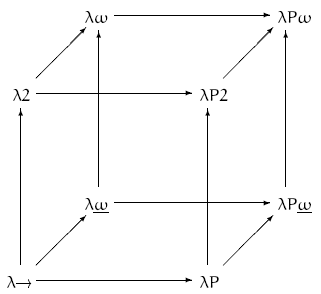
\includegraphics[width=0.5\textwidth]{img/Lambda_cube.png}
  \caption{Лямбда-куб}
\end{figure}

База куба -- просто типизированное $\lambda$-исчисление, в котором термы могут зависеть только от термов. Три оси соответствуют расширениям, комбинации которых позволяют получить остальные системы типов:

\begin{enumerate}
  \item Термы, которые зависят от типов -- система $\lambda2$ или \textbf{System F}
  \item Типы, которые зависят от типов -- система $\lambda \underline{\omega}$(операторы над типами)
  \item Типы, которые зависят от термов -- система $\lambda P$(зависимые типы)
\end{enumerate}

Затронув системы типизации лямбда-исчисления, нельзя не отметить так называемое соответствие Карри-Говарда~\cite{howard1980formulae}, которое устанавливает прямую связь между логикой и теорией типов. Логической связке соответствует конструкция в теории типов, а логическому утверждению -- тип. Доказательству того факта, что утверждение истинно, соответствует тогда доказательство того факта, что соответствующий этому утверждению тип населен. Иначе говоря, мы можем предъявить $\lambda$-терм соответствующего типа, чтобы доказать исходное утверждение. Для наглядности некоторые соответствия сведены в таблицу:

\begin{table}[H]
  \centering
  \begin{tabular}{| c | c |}
    \hline
    Высказывание $A$: & Тип $A$: \\
    \hline
    Тождественная истинна & $\top$(единичный тип) \\
    \hline
    Тождественная ложь & $\bot$(пустой тип без обитателей) \\
    \hline
    $\lnot A$(отрицание) & $A \to \bot$ \\
    \hline
    $A \land B$(конъюнкция) & $A \times B$(тип-произведение) \\
    \hline
    $A \lor B$(дизъюнкция) & $A \coprod B$(тип-сумма) \\
    \hline
    $A \to B$(импликация) & $A \to B$(тип функций из $A$ в $B$) \\
    \hline
    $\exists x.P(x)$ & $\Sigma (x : A) (P a)$(тип зависимых пар) \\
    \hline
    $\forall x.P(x)$ & $\Pi (x : A) \to (P a)$(тип зависимых функций) \\
    \hline
  \end{tabular}
  \caption{Соответствия высказываний в логике и конструкций в теории типов}
\end{table}

Чем больше логических связок мы хотим использовать, тем более мощные теории типов  нам придется использовать, чтобы доказывать эти утверждения. Так, например, если нам потребуется доказывать формулы пропозициональной логики, то мы можем обойтись просто типизированным $\lambda$-исчислением. Если нам понадобятся кванторы в формулах, то на помощь приходят теории с зависимыми типами.

Существует две известные теории с зависимыми типами -- исчисление конструкций(Calculus Of Constructions), представленное Тьерри Коканом в \cite{coquand1988calculus} и интуиционистская теория типов Мартин-Лёфа(Martin-L{\"o}f Type Theory), описанная в \cite{martin1975intuitionistic}. Их расширения лежат в основе таких систем интерактивного доказательства теорем как \textbf{Coq} и \textbf{Agda} соответственно.

\subsection{Мотивация}

Как уже упоминалось в введении, языки с зависимыми типами являют собой полноценную логику, позволяя использовать их как инструмент для формализации математики.

Это возможно благодаря соответствию Карри-Говарда, которое устанавливает связь между логикой и теорией типов. То есть, логической связке соответствует конструкция в теории типов, а логическому утверждению -- тип. Доказательству того факта, что утверждение истинно, соответствует тогда доказательство того факта, что соответствующий этому утверждению тип населен. Иначе говоря, мы можем предъявить терм соответствующего типа, чтобы доказать исходное утверждение. Сведем для наглядности некоторые соответствия в таблицу:

\begin{table}[H]
  \centering
  \begin{tabular}{| c | c |}
    \hline
    Высказывание $A$: & Тип $A$: \\
    \hline
    Тождественная истинна & $\top$(единичный тип) \\
    \hline
    Тождественная ложь & $\bot$(пустой тип без обитателей) \\
    \hline
    $\lnot A$(отрицание) & $A \to \bot$ \\
    \hline
    $A \land B$(конъюнкция) & $A \times B$(тип-произведение) \\
    \hline
    $A \lor B$(дизъюнкция) & $A \coprod B$(тип-сумма) \\
    \hline
    $A \to B$(импликация) & $A \to B$(тип функций из $A$ в $B$) \\
    \hline
    $\exists x.P(x)$ & $\Sigma (x : A) (P a)$(тип зависимых пар) \\
    \hline
    $\forall x.P(x)$ & $\Pi (x : A) \to (P a)$(тип зависимых функций) \\
    \hline
  \end{tabular}
  \caption{Соответствия высказываний в логике и конструкций в теории типов}
\end{table}
Чем больше логических связок мы хотим использовать, тем более мощные теории типов  нам придется использовать, чтобы доказывать эти утверждения. Так, например, если нам потребуется доказывать формулы пропозициональной логики, то мы можем обойтись просто типизированным $\lambda$-исчислением. Если нам понадобятся кванторы в формулах, то на помощь приходят теории с зависимыми типами.

Существует две известные теории с зависимыми типами -- исчисление конструкций(Calculus Of Constructions), представленное Тьерри Коканом в \cite{coquand1988calculus} и интуиционистская теория типов Мартин-Лёфа(Martin-L{\"o}f Type Theory), описанная в \cite{martin1975intuitionistic}. Их расширения лежат в основе таких систем интерактивного доказательства теорем как \textbf{Coq} и \textbf{Agda} соответственно. Нам сейчас не очень важно, чем именно отличаются эти две теории, поэтому мы не будем заострять на этом внимание.

Отметим, что для построения доказательств иногда бывает полезна функциональная экстенсиональность. Это конструкция, которая по двум функциям $f, g : X \to Y$ и доказательству $\forall x (f x \equiv g x)$ возвращает нам доказательство $f \equiv g$. В \textbf{Agda}, например, функциональной экстенсиональности нет -- её можно постулировать, однако сами авторы не рекомендуют использовать постулаты по той простой причине, что их использование позволяет, например, предъявить элемент пустого множества.

Нам хотелось бы строить доказательства, не используя таких <<неугодных>> с точки зрения языка конструкций. Незамедлительно возникает вопрос, есть такая теория типов(а еще лучше -- язык), в которой функциональная экстенсиональность была бы сконструирована должным образом, а не постулирована? Ответ -- да, есть.

% Написать про Vclang, Валерину теорию, дать ссылку(гитхаб?)

\subsection{Постановка задачи}

Целью работы является формализация различных представлений $\lambda$-термов. Для достижения этой цели необходимо решить следующие задачи:

\begin{enumerate}
  \item Определить интересующие нас представления лямбда-термов:
    \begin{enumerate}
      \item Именованное
      \item Неименованное
      \item Монадическое
    \end{enumerate}
  \item Для каждого представления определить операцию подстановки
  \item Для каждого представления доказать свойства операции подстановки:
    \begin{enumerate}
      \item Унитальность(наличие правой и левой единицы)
      \item Ассоциативность
    \end{enumerate}
  \item Установить соответствие между описанными в первом пункте представлениями
\end{enumerate}

Операция подстановки является фундаментальной операцией над термами. С её помощью вводятся отношения, которые наделяют $\lambda$-исчисление вычислительной семантикой, например $\beta$-редукция. Унитальность и ассоциативность -- её основные свойства, поэтому мы хотим формализовать именно эту операцию.

\subsection{Существующие решения}

Стоит отметить, что задача формализации $\lambda$-исчисления довольно популярна, в связи с чем существует довольно много её решений. Один из примеров -- \cite{lambdaForm}, в котором, в частности, формализовано чистое $\lambda$-исчисление.

Однако для этого, и аналогичных ему решений характерен тот факт, что авторы рассматривают лишь одно представление $\lambda$-термов, упуская из внимания остальные и, соответственно, не устанавливая между ними никакого соответствия.

TODO


\section{Представления \texorpdfstring{$\lambda$}{лямбда}-термов}

В этой главе мы опишем три представления $\lambda$-термов: именованное, неименованное(через индексы Де Брауна) и монадическое. Мы формально опишем, как определяются термы в каждом из представлений, определим характерные свойства для каждого представления и покажем, почему они верны. Кроме того, мы установим соответствие между всеми представлениями.

\subsection{Именованное представление термов}
\label{sec:named}

Термы $\lambda$-исчисления($\lambda$-термы) в именованном представлении конструируются из переменных путем применения друг к другу или создания анонимных функций.

Формально, пусть $\mathcal{V}=\{x,y,z,\dots\}$ -- счетное множество переменных. Договоримся обозначать переменные прописными буквами, а произвольные термы -- заглавными. Тогда множество $\lambda$-термов $\Lambda$ определяется индуктивно, согласно следующим правилам:
\begin{center}
  \AxiomC{$v \in \mathcal{V}$}
  \UnaryInfC{$v \in \Lambda$}
  \DisplayProof{}
\end{center}

\begin{center}
  \AxiomC{$M \in \Lambda$}
  \AxiomC{$N \in \Lambda$}
  \BinaryInfC{$M N \in \Lambda$}
  \DisplayProof{}
\end{center}

\begin{center}
  \AxiomC{$M \in \Lambda$}
  \AxiomC{$v \in \mathcal{V}$}
  \BinaryInfC{$\lambda v.M \in \Lambda$}
  \DisplayProof{}
\end{center}

Нотация аппликации $M N$ обозначает применение функции $M$ ко входу $N$. Заметим, что так как здесь не вводится никаких правил типизации, то ничто не мешает нам применить терм к самому себе(i.e $F F$). Нотация абстракции $\lambda x.M$, в свою очередь, обозначает создание анонимной функции от переменной $x$, которая сопоставляет конкретному значению $x$ выражение $M[x]$. Здесь заметим, что терм $M$ вовсе не обязан содержать в себе переменную $x$, в таком случае мы считаем абстракцию $\lambda x.M$ константной функцией.

Некоторые примеры термов:
\begin{gather*}
   \lambda x.x \\
   \lambda x y.x \\
   (\lambda x.f (x x)) (\lambda x.f (x x))
\end{gather*}

Переменная $x$ после абстракции $\lambda x.M$ называется \textit{связанной}. Соответственно, до абстракции она была \textit{свободной}. Формально, множества $FV(T)$ свободных и $BV(T)$ связанных переменных терма $T$ определяются индуктивно следующим образом:
\begin{align*}
  FV(x) &= \{x\} \\
  FV(M N) &= FV(M) \cup FV(N) \\
  FV(\lambda x. M) &= FV(M) \setminus \{x\} \\
  \\
  BV(x) &= \emptyset \\
  BV(M N) &= BV(M) \cup BV(N) \\
  BV(\lambda x. M) &= \{x\} \cup BV(M)
\end{align*}

Применение абстракции к некоторому аргументу $(\lambda x.M) N$ -- это \textit{подстановка} $M[x \mapsto N]$ терма $N$ вместо \textit{свободных} вхождений переменной $x$ в терме $M$. Формально, правила подстановки:
\begin{align*}
  x[x \mapsto N] &= N \\
  y[x \mapsto N] &= y, (x \neq y) \\
  (T S)[x \mapsto N] &= T[x \mapsto N] S[x \mapsto N] \\
  (\lambda x.T)[x \mapsto N] &= \lambda x.T \\
  (\lambda y.T)[x \mapsto N] &= \lambda y.T[x \mapsto N], (y \notin FV(N), x \neq y)
\end{align*}

Рассмотрим, что произойдет, если в последнем правиле условие $ y \notin FV(N)$ не выполняется:
$$ (\lambda y.x)[x \mapsto y] = \lambda y.y $$

Получилось, что в результате подстановки мы превратили константную функцию $\lambda y.x$ в тождественную. Такая ситуация называется проблемой захвата переменной, когда при подстановке в $\lambda$-абстракцию переменные подставляемого терма захватываются абстракцией.

Эту проблему можно решить если принять так называемое соглашение Барендрегта о том, что имена связанных переменных всегда выбирать так, чтобы они отличались от имен свободных. В примере выше, например, мы можем переименовать связанную переменную $y$ в свежую $z$ и поведении абстракции $\lambda z.x$ не изменится. Тогда подстановку можно использовать без каких-либо оговорок о свободных и связанных переменных. Пример выше превратится в:
$$ (\lambda z.x)[x \mapsto y] = \lambda z.y $$

Как мы уже установили выше, мы можем переименовывать связанные переменные в абстракциях и их поведение при применении к аргументам не изменится. Более того, имена связанных переменных не играют для нас никакой роли. Поэтому, как правило, $\lambda$-термы и рассматривают с точностью до имен параметров абстракций. Формально, на множестве именованных термов $\Lambda$ можно задать отношение $\alphaeq \in \Lambda \times \Lambda$, которое называется $\alpha$-эквивалентностью и определяется как минимальное отношение конгруэнтности, порожденное следующими правилами:

\begin{center}
  \AxiomC{$x \in \mathcal{V}$}
  \UnaryInfC{$x \alphaeq x$}
  \DisplayProof{}
\end{center}

\begin{center}
  \AxiomC{$M \alphaeq M'$}
  \AxiomC{$N \alphaeq N'$}
  \BinaryInfC{$M N \alphaeq M' N'$}
  \DisplayProof{}
\end{center}

\begin{center}
  \AxiomC{$M[x \mapsto y] \alphaeq M'$}
  \AxiomC{$y \notin FV(M)$}
  \BinaryInfC{$\lambda x. M \alphaeq \lambda y.M'$}
  \DisplayProof{}
\end{center}

Наконец, сформулируем лемму о подстановке:

\begin{prop}
  \label{named:assoc}
  Для любых $T, M, N \in \Lambda; x, y \in \mathcal{V}$, если $x \neq y$ и $x \notin FV(M)$, то верно $T[x \mapsto N][y \mapsto M] = T[y \mapsto M][x \mapsto N[y \mapsto M]]$
\end{prop}

\begin{proof}
  Индукция по терму $T$. База индукции -- случай, когда $T$ является переменной. Рассмотрим три случая:
  \begin{enumerate}
    \item $T \equiv x$. Левая часть -- $x[x \mapsto N][y \mapsto M] = N[y \mapsto M]$. Правая часть -- $x[y\mapsto M][x \mapsto N[y \mapsto M]] = N[y \mapsto M]$.
    \item $T \equiv y$. Левая часть -- $y[x \mapsto N][y \mapsto M] = M$. Правая часть -- $y[y\mapsto M][x \mapsto N[y \mapsto M]] = M[x\mapsto N[y \mapsto M]]$. Так как $x \notin FV(M)$, то $M[x\mapsto N[y \mapsto M]] = M$
    \item $T \equiv z \neq x,y$. Обе части редуцируются к $z$.
  \end{enumerate}

  Случай аппликации тривиален, рассмотрим случай абстракции $\lambda z.T$. Рассмотрим возможные случаи:

  \begin{enumerate}
    \item $z \equiv x$. Левая часть -- $(\lambda x.T)[x \mapsto N][y \mapsto M] = (\lambda x.T)[y \mapsto M] \overset{\mathrm{x \notin FV(M)}}{=} \lambda x.T[y \mapsto M]$. Правая часть -- $(\lambda x.T)[y \mapsto M][x \mapsto N[y \mapsto M]] \overset{\mathrm{x \notin FV(M)}}{=} (\lambda x.T[y \mapsto M])[x \mapsto N[y \mapsto M]] = \lambda x.T[y \mapsto M]$.

    \item $z \equiv y$. Пусть $y \in FV(N)$ и $y \in FV(M)$. По соглашению Барендрегта, нам нужно переименовать $y$ в свежую переменную $y'$, такую что $y' \notin FV(N)$ и $y' \notin FV(M)$. Это эквивалентно тому, что мы можем осуществить подстановку $\lambda y'.t[y \mapsto y']$. Вычислим левую часть:
    \begin{gather*}
      (\lambda y'.T[y \mapsto y'])[x \mapsto N][y \mapsto M] = \\
       \lambda y'.T[y \mapsto y'][x \mapsto N][y \mapsto M] \overset{\mathrm{IH}}{=} \\
       \lambda y'.T[y \mapsto y'][y \mapsto M][x \mapsto N[y \mapsto M]]
    \end{gather*}

    Правая часть:
    \begin{gather*}
      (\lambda y'.T[y \mapsto y'])[y \mapsto M][x \mapsto N[y \mapsto M]] = \\
      \lambda y'.T[y \mapsto y'][y \mapsto M][x \mapsto N[y \mapsto M]]
    \end{gather*}

    Заметим здесь, что так как $y' \notin FV(N)$ и $y' \notin FV(M)$, то, очевидно, что $y' \notin FV(N[y \mapsto M])$, поэтому в последнем переходе обе подстановки <<проваливаются>> в абстракцию.

    \item $z \equiv y$. Пусть $y \in FV(N)$, но теперь уже $y \notin FV(M)$. Аналогично предыдущему пункту, мы переименовываем $y$ в свежую переменную $y'$, такую что $y' \notin FV(N)$ и $y' \notin FV(M)$, осуществляя подстановку $\lambda y'.t[y \mapsto y']$. Вычислим левую часть:
    \begin{gather*}
      (\lambda y'.T[y \mapsto y'])[x \mapsto N][y \mapsto M] = \\
       \lambda y'.T[y \mapsto y'][x \mapsto N][y \mapsto M] \overset{\mathrm{IH}}{=} \\
       \lambda y'.T[y \mapsto y'][y \mapsto M][x \mapsto N[y \mapsto M]]
    \end{gather*}

    А в этом случае, заметим, что так как мы сначала заменили \textbf{все} свободные вхождения $y$ в $T$ на $y'$, а потом на место $y$ подставили $M$, то вторая подстановка ничего не делает, поэтому левая часть окончательно равна $\lambda y'.T[y \mapsto y'][x \mapsto N[y \mapsto M]]$

    Правая часть тогда редуцируется в:
    \begin{gather*}
      (\lambda y.T)[y \mapsto M][x \mapsto N[y \mapsto M]] = \\
      (\lambda y.T)[x \mapsto N[y \mapsto M]] = \\
      \lambda y.T[x \mapsto N[y \mapsto M]]
    \end{gather*}

    В последнем шаге вычисления, отметим, что так как $y \in FV(N)$ и $y \notin FV(M)$, то $y \notin FV(N[y \mapsto M])$, поэтому подстановка снова заносится под абстракцию. Переименуем и здесь $y$ в $y'$, тогда получим:
    \begin{gather*}
      \lambda y.T[x \mapsto N[y \mapsto M]] \alphaeq \\
      \lambda y'.T[x \mapsto N[y \mapsto M]][y \mapsto y'] \overset{\mathrm{IH}}{=} \\
      \lambda y'.T[y \mapsto y'][x \mapsto N[y \mapsto M][y \mapsto y']]
    \end{gather*}

    Из тех же соображений, что и выше, подстановка $N[y \mapsto M][y \mapsto y']$ -- это то же самое, что и $N[y \mapsto M]$, поэтому правая часть окончательно вычисляется в $\lambda y'.T[y \mapsto y'][x \mapsto N[y \mapsto M]]$.

    \item $z \neq x,y$. Доказательство аналогично предыдущим двум пунктам. \qedhere

  \end{enumerate}
\end{proof}

\subsection{Неименованное представление термов}
\label{sec:index}
Как уже мы уже видели в предыдущем разделе, имена формальных параметров $\lambda$-абстракций не важны и, в целом, мы можем не обращать на них внимания. Более того, мы можем вообще отказаться от именованных переменных! Широко известен альтернативный способ записи термов через так называемые индексы Де Брауна(De Bruijn) -- \cite{nikolas1972bruijn}. В нем вместо имен переменных используются числовые индексы, показывающие сколько лямбд назад была захвачена переменная. Например комбинатор $S = \lambda f g x. f x (g x)$, записанный в таком представлении будет иметь следующий вид: $\lambda(\lambda(\lambda 3 1 (2 1)))$.

Существует и альтернативный способ такого представления. Множество всех термов разбивается на так называемые <<уровни>>(levels) и вместо него рассматриваются множества $\Lambda_{n}$, где $n$ -- длина контекста, в котором определен терм. О контексте в котором определен терм, можно думать, как о простом списке свободных переменных терма. Индуктивно, они определяются следующим образом:

\begin{center}
  \AxiomC{$0 \leqslant i < n$}
  \UnaryInfC{$v_{n, i} \in \Lambda_{n}$}
  \DisplayProof{}
\end{center}

\begin{center}
  \AxiomC{$T_{1} \in \Lambda_{n}$}
  \AxiomC{$T_{2} \in \Lambda_{n}$}
  \BinaryInfC{$T_{1} T_{2} \in \Lambda_{n}$}
  \DisplayProof{}
\end{center}

\begin{center}
  \AxiomC{$T \in \Lambda_{n + 1}$}
  \UnaryInfC{$\lambda T \in \Lambda_{n}$}
  \DisplayProof{}
\end{center}

В случае переменной индекс $i$ обозначает позицию переменной в контексте. Договоримся отсчитывать ее с конца контекста. Комбинатор $S$, например, в таком представлении будет выглядеть вот так: $\lambda (\lambda (\lambda v_{3,2} v_{3, 0} (v_{3, 1} v_{3, 0})))$.

Такое представление термов удобно потому что $\alpha$-эквивалентность сводится к самому обычному равенству и, как следствие, пропадает проблема коллизии имен переменных.

Определим операцию подстановки для таких термов. Мы определим ее в более общем случае -- вместо какой-то одной переменной мы будем осуществлять подстановку во \textbf{все} переменные терма. Пусть $T \in \Lambda_{n}$, и $S_{0}, \dots S_{n-1} \in \Lambda_{k}$. Тогда $subst(T, S_{n - 1}, \dots, S_{0}) \in \Lambda_{k}$ определяется следующим образом:
\begin{gather*}
  subst(v_{n, i}, S_{n - 1}, \dots, S_{0}) = S_{i} \\
  subst(T, v_{n, n-1}, \dots, v_{n, 0}) = T \\
  subst(T_{1} T_{2}, S_{n - 1}, \dots, S_{0}) = \\
  subst(T_{1}, S_{n - 1}, \dots, S_{0})\ subst(T_{2}, S_{n - 1}, \dots, S_{0}) \\
  subst(\lambda T, S_{n - 1}, \dots, S_{0}) = \lambda (subst(T, w(S_{n - 1}), \dots, w(S_{0}), v_{n+1, 0})
\end{gather*}

Операция $w(T)$ работает следующим образом. Пусть терм $T \in \Lambda_{n}$, тогда терм $w(T) \in \Lambda_{n+1}$ и определен как:
\begin{gather*}
  w(v_{n, i}) = v_{n+1, i+1} \\
  w(T_{1} T_{2}) = w(T_1)\ w(T_2) \\
  w(\lambda T) = \lambda (w(T))
\end{gather*}

Сформулируем и докажем вспомогательную лемму, которая пригодится нам далее:
\begin{lemma}
  \label{index:weak_lemma}
  Пусть $T \in \Lambda_{n}$, а $S_{n-1}, \dots, S_{0} \in \Lambda_{m}$. Тогда $subst(w(T), w(S_{n-1}), \dots, w(S_{0}), v_{m+1, 0}) = w(subst(T, S_{n-1}, \dots S_{0}))$
\end{lemma}

\begin{proof}
  Индукция по структуре терма $T$.
  \begin{enumerate}
    \item База индукции -- $v_{n, i}$. Левая часть равна, по определению подстановки:
    $$ subst(v_{n+1, i+1}, w(S_{n-1}), \dots, w(S_{0}), v_{m+1, 0}) = w(S_{i})$$
    Правая часть:
    $$w(subst(v_{n,i}, S_{n-1}, \dots, S_{0})) = w(S_{i})$$

    \item Случай аппликации снова тривиален. Рассмотрим случай абстракции $\lambda T$. Левая часть вычислится в:
    \begin{gather*}
        subst(w(\lambda T), w(S_{n-1}), \dots, w(S_{0}), v_{m+1, 0}) = \\
        subst(\lambda w(T), w(S_{n-1}), \dots, w(S_{0}), v_{m+1, 0}) = \\
        \lambda subst(w(T), w(w(S_{n-1})), \dots, w(w(S_{0})), v_{m+2, 1}, v_{m+2,0}) \overset{\mathrm{IH}}{=} \\
        \lambda w(subst(T, w(S_{n-1}), \dots, w(S_{0}), v_{m+1, 0}))
    \end{gather*}

    Правая часть вычисляется в:
    \begin{gather*}
        w(subst(\lambda T, S_{n-1}, \dots, S_{0})) = \\
        w(\lambda subst(T, w(S_{n-1}), \dots, w(S_{0}), v_{m+1, 0})) =
        \lambda w(subst(T, w(S_{n-1}), \dots, w(S_{0}), v_{m+1, 0}))
    \end{gather*}
  \end{enumerate}
\end{proof}

Аналогично именованному представлению, сформулируем лемму о подстановке:

\begin{prop}
  \label{index:assoc}
  Пусть $T \in \Lambda_{n}; T_{n - 1}, \dots T_{0} \in \Lambda_{m}, S_{m-1}, \dots S_{0} \in \Lambda_{k}$, тогда верно $subst(subst(T, T_{n - 1}, \dots T_{0}), S_{m-1}, \dots S_{0}) = subst(T, T_{n - 1}' \dots, T_{0}')$, где $T_{i}' = subst(T_{i}, S_{m-1}, \dots S_{0})$.
\end{prop}

Заметим еще, что в таком представлении термов нет необходимости в сторонних условиях, как в лемме о подстановке для именованных термов.

\begin{proof}
  Это утверждение точно так же доказывается индукцией по структуре терма $T$. База индукции -- случай, когда терм представляет собой переменную $v_{n, i}$. Тогда левая часть вычисляется в $subst(T_{i}, S_{m-1}, \dots S_{0})$, ровно как и правая.

  Случай аппликации снова тривиален, рассмотрим случай абстракции $\lambda T$. Вычислим левую часть:
  \begin{gather*}
    subst(subst(\lambda T, T_{n-1}, \dots, T_{0}), S_{m-1}, \dots, S_{0}) = \\
    subst(\lambda subst( T, w(T_{n - 1}), \dots w(T_{0}), v_{m+1, 0} ), S_{m - 1}, \dots, S_{0}) = \\
    \lambda(subst(subst( T, w(T_{n - 1}), \dots w(T_{0}), v_{m+1, 0} ), w(S_{m-1}), \dots, w(S_{0}), v_{k+1, 0}) \overset{\mathrm{IH}}{=} \\
    \lambda(subst(T, subst(w(T_{n-1}), w(S_{m-1}), \dots, w(S_{0}), v_{k+1, 0}), \dots, \\
    subst(w(T_{0}), w(S_{m-1}), \dots, w(S_{0}), v_{k+1, 0}), subst(v_{m+1, 0}, w(S_{m-1}), \dots, w(S_{0}), v_{k+1, 0}))) = \\
    \lambda(subst(T, subst(w(T_{n-1}), w(S_{m-1}), \dots, w(S_{0}), v_{k+1, 0}), \dots, \\
    subst(w(T_{0}), w(S_{m-1}), \dots, w(S_{0}), v_{k+1, 0}), v_{k+1, 0}))
  \end{gather*}

  Вычислим теперь правую часть:
  \begin{gather*}
    subst(\lambda T, subst(T_{n-1}, S_{m - 1}, \dots, S_{0}), \dots, subst(T_{0}, S_{m - 1}, \dots, S_{0})) = \\
    \lambda(subst(T, w(subst(T_{n-1}, S_{m - 1}, \dots, S_{0})), \dots, w(subst(T_{0}, S_{m - 1}, \dots, S_{0})), v_{k+1, 0}))
  \end{gather*}

  По лемме~\ref{index:weak_lemma} $subst(w(T_{i}), w(S_{m-1}), \dots, w(S_{0}), v_{k+1, 0}) = w(subst(T_{i}, S_{m - 1}, \dots, S_{0}))$ для всех $i=\overline{0, n-1}$, следовательно наше утверждение верно.
\end{proof}

\subsection{Монадическое представление термов}
\label{sec:monad}
Существует еще один способ записи $\lambda$-термов, описанный в \cite{bird1999bruijn}. Библиотека \textbf{Bound}~\cite{bound} для языка \textbf{Haskell}, например, использует именно монадическое представление.

Основная идея в том, что именованное представление для термов можно обобщить и свободные переменные брать из произвольного множества $V$. Тогда множество термов $\Lambda_{V}$ определяется индуктивно по следующим правилам:
\begin{center}
  \AxiomC{$v \in V$}
  \UnaryInfC{$v \in \Lambda_{V}$}
  \DisplayProof{}
\end{center}

\begin{center}
  \AxiomC{$M \in \Lambda_{V}$}
  \AxiomC{$N \in \Lambda_{V}$}
  \BinaryInfC{$M N \in \Lambda_{V}$}
  \DisplayProof{}
\end{center}

\begin{center}
  \AxiomC{$M \in \Lambda_{V \coprod \{*\}}$}
  \UnaryInfC{$\lambda M \in \Lambda_{V}$}
  \DisplayProof{}
\end{center}

Здесь $\{*\}$ -- это произвольное одноэлементное множество, а $\coprod$ -- операция размеченного объединения множеств. По определению $A \coprod B$ состоит из элементов $inl(a)$ и $inr(b)$, где $a \in A$ и $b \in B$.  Так как для абстракции нам нужно иметь на одну свободную переменную больше, то ее можно получить взяв размеченное объединение с произвольным одноэлементным множеством. Это представление так же удобно для компьютерной реализации за счет того, что проверку корректности построения термов можно выполнять на уровне типов.

Пусть у нас есть функция $f : V \to W$, тогда мы можем задать функцию $F_{f}$ из $\Lambda_{V}$ в $\Lambda_{W}$ рекурсией по терму $T \in \Lambda_{V}$:

\begin{enumerate}
  \item $v \mapsto f(v)$
  \item $M\ N \mapsto F_{f}(M)\ F_{f}(N)$
  \item $\lambda M \mapsto \lambda F_{f'(f)}(M)$. Заметим, что просто так отобразить терм $M$ с помощью функции $f$ мы не можем, так как ее домен не совпадает со множеством, которым параметризован тип терма $M$. Поэтому мы построим по $f$ функцию $f'(f) : V \coprod \{*\} \to W \coprod \{*\}$. Устроена она будет следующим образом:
  \begin{enumerate}
    \item $f'(f)(inl(x)) = inl(f(x))$
    \item $f'(f)(inr(*)) = inr(*)$
  \end{enumerate}
\end{enumerate}

Знакомый с языком программирования \textbf{Haskell} или теорией категорий читатель узнает, что мы задали структуру функтора. Интуитивно, действие этого функтора -- это переименование переменных. Покажем, что это действительно функтор, именно, что он уважает тождественное отображение и композицию отображений.

\begin{prop}
  \label{monad:fmap-resp-id}
  Для любого $T \in \Lambda_{V}$ верно, что $F_{id_{V}}(T) = T$
\end{prop}

\begin{proof}
  Индукция по терму $T$. База тривиальна, равно как и случай аппликации, покажем, что утверждение верно и для случая лямбды. Вспомогательная функция $f'(f)$ устроена следующим образом:
  \begin{enumerate}
    \item $f'(id_{V})(inl(x)) = inl(x)$
    \item $f'(id_{V})(inr(*)) = inr(x)$
  \end{enumerate}
  Следовательно, оно является тождеством на $V \coprod \{*\}$. По индукционной гипотезе получаем, что случай для лямбды тоже верен.

  Формальное доказательство этого утверждения можно увидеть в приложении~\ref{apendix:monad}, в функции \texttt{fmap-respects-id}
\end{proof}

\begin{prop}
  \label{monad:fmap-resp-comp}
  Для любого $T \in \Lambda_{V}$ и $f : V \to W$, $g : W \to X$ верно, что $F_{g \circ f}(T) = F_{g}(T) \circ F_{f}(T)$
\end{prop}

\begin{proof}
  Снова индукция по терму $T$. Случай переменной снова тривиален, случай аппликации напрямую следует из индукционной гипотезы, рассмотрим случай абстракции. Посмотрим, во что вычислится левая часть:
  \begin{gather*}
    F_{g \circ f}(\lambda M) = \lambda F_{f'(g \circ f)}(M) \\
    \text{где} \\
    f'(g \circ f)(inl(v)) = inl(g(f(v))) \\
    f'(g \circ f)(inr(*)) = inr(*)
  \end{gather*}

  Правая, в свою очередь:
  \begin{gather*}
    F_{g}(F_{f}(\lambda M)) = F_{g}(\lambda F_{f'(f)}(M)) = \\
    \lambda F_{g'(g)}(F_{f'(f)}(M))
  \end{gather*}

  Вспомогательная функция $f'(f) : V \coprod \{*\} \to W \coprod \{*\}$ устроена здесь следующим образом:
  \begin{enumerate}
    \item $f'(f)(inl(v)) = inl(f(v))$
    \item $f'(f)(inr(*)) = inr(*)$
  \end{enumerate}

  Вспомогательная функция $g'(g) : W \coprod \{*\} \to X \coprod \{*\}$ устроена здесь следующим образом:
  \begin{enumerate}
    \item $g'(g)(inl(w)) = g'(g)(inl(f(v))) = inl(g(f(v)))$
    \item $g'(g)(inr(*)) = inr(*)$
  \end{enumerate}

  Несложно увидеть, что эти две функции из левой и правой частей ведут себя одинаково, следовательно и для случая лямбды утверждение верно.
  Формальное доказательство этого утверждения можно увидеть в приложении~\ref{apendix:monad}, в функции \texttt{fmap-respects-сomp}
\end{proof}

Мы пойдем еще дальше и зададим структуру монады. Существует много способов определить её, мы воспользуемся тем, который принят в языке программирования \textbf{Haskell}. Именно, мы определим две операции: монадическую единицу $\texttt{return} : V \to \Lambda_{V}$ и монадическое связывание $\texttt{bind} : \Lambda_{V} \to (V \to \Lambda_{W}) \to \Lambda_{W}$. Кроме этого, мы покажем, что они удовлетворяют монадическим законам.

Монадическая единица устроена очень просто -- это переменная. Связывание же, принимает на вход так называемую стрелку Клейсли~\cite{kleisliArrows} $k : V \to \Lambda_{W}$ и определяется индуктивно по структуре терма $T$:

\begin{enumerate}
  \item $v \mapsto k(v)$
  \item $M\ N \mapsto (\texttt{bind}(M, k))\ (\texttt{bind}(N, k))$
  \item $\lambda M \mapsto \lambda(\texttt{bind}(M, k'(k)))$, где $k'(k) : V \coprod \{*\} \to \Lambda_{W \coprod \{*\}}$ и определяется следующим образом:
    \begin{enumerate}
      \item $k'(k)(inl(v)) = F_{inl}(k(v))$
      \item $k'(k)(inr(*)) = \texttt{return}(inr(*))$
    \end{enumerate}
\end{enumerate}


Сформулируем и докажем теперь свойства этих двух операций.

\begin{prop}
  \label{monad:bind-right-unit}
  Для любого $T \in \Lambda_{V}$ верно $\texttt{bind}(T, \texttt{return}) = T$.
\end{prop}

\begin{proof}
  Индукция по структуре терма $T$:
  \begin{enumerate}
    \item База индукции, $T = v$. Имеем, что $\texttt{bind}(v, \texttt{return}) = \texttt{return}(v) = v$.
    \item Случай аппликации напрямую следует из предположения индукции.
    \item Пусть теперь $T = \lambda M$. Имеем, что $\texttt{bind}(\lambda M, \texttt{return}) = \lambda (\texttt{bind}(M, k'(\texttt{return})))$. Вспомогательное отображение $k'(return)$ устроено следующим образом:
    \begin{enumerate}
      \item $k'(\texttt{return})(inl(v)) = F_{inl}(\texttt{return}(v)) = \texttt{return}(inl(v))$
      \item $k'(\texttt{return})(inr(*)) = \texttt{return}(inr(*))$
    \end{enumerate}
  \end{enumerate}

  Заметим, что оно ведет себя так же, как и \texttt{return} на $V \coprod \{*\}$, следовательно по индукционной гипотезе получаем исходное утверждение.
  Формальное доказательство этого утверждения можно увидеть в приложении~\ref{apendix:monad}, в функции \texttt{bind-right-unit}.
\end{proof}

\begin{prop}
  \label{monad:bind-left-unit}
  Для любого $v \in V$ и $k : V \to \Lambda_{V}$ верно $\texttt{bind}(\texttt{return}(v), k) = k(v)$
\end{prop}

\begin{proof}
  Утверждение тривиально следует из определения \texttt{bind} и того факта, что \texttt{return} -- это переменная. Формальное доказательство этого утверждения можно увидеть в приложении~\ref{apendix:monad}, в функции \texttt{bind-left-unit}.
\end{proof}

Прежде, чем формулировать последний монадный закон, сформулируем и докажем несколько технических лемм, которые помогут нам в его доказательстве.

\begin{lemma}
  \label{monad:bind-fmap-comm-lhs}
  Для любых $T \in \Lambda_{V}$, $f : V \to W$ и $k : W \to \Lambda_{U}$ верно $\texttt{bind}(F_{f}(T), k) = \texttt{bind}(T, k \circ f)$.
\end{lemma}

\begin{proof}
  Индукция по структуре терма $T$ с тривиальными случаями переменной и аппликации. Рассмотрим случай абстракции $\lambda M$. Нам нужно показать, что $\lambda \texttt{bind}(F_{f'(f)}(M), k'(k)) = \lambda \texttt{bind}(M, k'(k \circ f))$. По индукционной гипотезе мы знаем, что $\texttt{bind}(F_{f'(f)}(M), k'(k)) = \texttt{bind}(M, k'(k) \circ f'(f))$, Заметим теперь, что $k'(k \circ f)$ и $k'(k) \circ f'(f)$ ведут себя одинаково на всех входах, следовательно это утверждение доказано. Формальное доказательство этого утверждения можно увидеть в приложении~\ref{apendix:monad}, в функции \texttt{bind-fmap-comm-lhs}.
\end{proof}

\begin{lemma}
  \label{monad:bind-fmap-comm-rhs}
  Для любых $T \in \Lambda_{V}$, $f : W \to U$ и $k : V \to \Lambda_{W}$ верно $ F_{f}(\texttt{bind}(T, k)) = \texttt{bind}(T, (x \mapsto F_{f}(k(x))))$.
\end{lemma}

\begin{proof}
  Снова индукция по структуре терма $T$. Случай переменной и аппликации снова тривиален, поэтому рассмотрим случай абстракции $\lambda M$.

  Нам нужно показать, что $\lambda F_{f'(f)}(\texttt{bind}(M, k'(k))) = \lambda \texttt{bind}(M, k'(x \mapsto F_{f}(k(x))))$. По индукционной гипотезе мы знаем, что $F_{f'(f)}(\texttt{bind}(M, k'(k))) = \texttt{bind}(M, (x \mapsto F_{f'(f)}(k'(k)(x))))$. Покажем теперь, что стрелки Клейсли $ k'(x \mapsto F_{f}(k(x))) $ и $ x \mapsto F_{f'(f)}(k'(k)(x)) $ ведут себя одинаково на всех входах:

  \begin{enumerate}
    \item $inr(*)$. Обе стрелки вычисляются в $\texttt{return}(inr(*))$
    \item $inl(v)$. Надо показать, что $F_{f'(inl)}(F_{f}(k(v))) = F_{f'(f)}(F_{inl}(k(v)))$. Так как $\Lambda_{-}$ -- функтор и он уважает композицию отображений имеем, что нужно показать $F_{f'(inl) \circ f}(k(v)) = F_{f'(f) \circ inl}(k(v))$. Для этого в свою очередь нужно снова показать, что два отображения $f'(inl) \circ f$ и $f'(f) \circ inl$ ведут себя одинаково на всех входах, но это очень легко понять, просто взглянув на определение $f'$.
  \end{enumerate}

  Формальное доказательство этого утверждения можно увидеть в приложении~\ref{apendix:monad}, в функции \texttt{bind-fmap-comm-rhs}.
\end{proof}

\begin{lemma}
  \label{monad:bind-fmap-comm}
  Для любого $T \in \Lambda_{V}$ и $f : V \to \Lambda_{W}$ верно $\texttt{bind}(F_{inl}(t), k'(g)) = F_{inl}(\texttt{bind}(T, f))$.
\end{lemma}

\begin{proof}
  Снова индукция по структуре терма $T$, случай переменной и аппликации тривиален, рассмотрим случай абстракции $\lambda M$.

  Левая часть вычислится в:
  $$ \lambda F_{f'(inl)}(\texttt{bind}(M, k'(f))) $$
  Правая в:
  $$ \lambda \texttt{bind}(F_{f'(inl)}(M), k'(k'(f))) $$

  По лемме~\ref{monad:bind-fmap-comm-lhs} имеем, что $\texttt{bind}(F_{f'(inl)}(M), k'(k'(f))) = \texttt{bind}(M, k'(k'(f)) \circ f'(inl))$. По лемме~\ref{monad:bind-fmap-comm-rhs} имеем $F_{f'(inl)}(\texttt{bind}(M, k'(f))) = \texttt{bind}(M, (x \mapsto F_{f'(inl)}(k'(f)(x))))$. Заметим теперь, что стрелки Клейсли $k'(k'(f)) \circ f'(inl)$ и $x \mapsto F_{f'(inl)}(k'(f)(x))$ ведут себя одинаково на всех входах, тогда по симметричности и транзитивности равенства получаем доказательство требуемого утверждения.

  Формальное доказательство этого утверждения можно увидеть в приложении~\ref{apendix:monad}, в функции \texttt{bind-fmap-comm}.
\end{proof}

\begin{prop}
  \label{monad:bind-assoc}
  Для любого $T \in \Lambda_{V}$, $f : V \to \Lambda_{W}, g : W \to \Lambda_{U}$ верно $\texttt{bind}(\texttt{bind}(T, f), g) = \texttt{bind}(T, (x \mapsto \texttt{bind}(f(x), g)) )$.
\end{prop}

\begin{proof}
  Индукция по терму $T$:
  \begin{enumerate}
    \item Рассмотрим случай, когда $T = v$. Тогда левая часть вычисляется в $\texttt{bind}(f(v), g)$, ровно как и правая.
    \item Случай для аппликации следует напрямую из индукционной гипотезы.
    \item Рассмотрим случай абстракции $\lambda M$. Посмотрим, во что вычисляется левая часть:
    \begin{gather*}
      \texttt{bind}(\texttt{bind}(\lambda M, f), g) = \texttt{bind}(\lambda \texttt{bind}(M, k'(f)), g) = \\
      \lambda \texttt{bind}(\texttt{bind}(M, k'(f)), k'(g)) \\
      \text{где} \\
      k'(g)(inl(w)) = F_{inl}(g(w)) \\
      k'(g)(inr(*)) = \texttt{return}(inr(*)) \\
      \text{и} \\
      k'(f)(inl(v)) = F_{inl}(f(v)) \\
      k'(f)(inr(*)) = \texttt{return}(inr(*))
    \end{gather*}

    Правая часть, в свою очередь, вычисляется в:
    \begin{gather*}
      \texttt{bind}(\lambda M, (x \mapsto \texttt{bind}(f(x), g))) = \lambda \texttt{bind}(M, k'(x \mapsto \texttt{bind}(f(x), g)))
    \end{gather*}

    Чтобы воспользоваться индукционной гипотезой, необходимо показать, что $k'(x \mapsto \texttt{bind}(f(x), g)) : V \coprod \{*\} \to \Lambda_{U \coprod \{*\}}$ ведет себя так же как и $x \mapsto \texttt{bind}(k'(f)(x), k'(g))$. Для этого мы просто покажем, что они возвращают одинаковый результат на всех входах.

    Рассмотрим два случая, как могут выглядеть входные данные:
    \begin{enumerate}
      \item $inr(*)$. Обе части вычисляются в $\texttt{return}(inr(*))$.
      \item $inl(v)$. Левая часть вычисляется в: $$ F_{inl}(\texttt{bind}(f(v), g)) $$
      Правая: $$\texttt{bind}(F_{inl}(f(v)), f'(g))$$
      Воспользовавшись леммой~\ref{monad:bind-fmap-comm} для терма $f(v)$ и $g$ получаем доказательство исходного утверждения. \qedhere
    \end{enumerate}
  \end{enumerate}

  Формальное доказательство этого утверждения можно увидеть в приложении~\ref{apendix:monad}, в функции \texttt{bind-assoc}.
\end{proof}


Отметим наконец, что действие функтора мы проинтерпретировали, как переименование переменных. Действие монадического связывания можно, в таком случае, проинтерпретировать как подстановку. Это утверждение не столь очевидно, но если рассмотреть сигнатуру \texttt{bind} и обратить внимание на то, что функцию $k : V \to \Lambda_{W}$ можно задать в виде списка пар $(V, \Lambda_{W})$, то это соответствие становится куда более явным. Монадные законы, в свою очередь, в точности описывают свойства подстановки, которые мы в явном виде задали в прошлых разделах~\ref{sec:named} и \ref{sec:index}.

\subsection{Преобразования между представлениями}
\label{sec:conversions}
В этом разделе мы опишем преобразования между представлениями и начнем с преобразования именованных термов в неименованные. Очевидно, что для осуществления этого нам необходимо знать порядок на переменных в терме. Поэтому мы считаем, что кроме самого терма нам дают контекст.

\begin{definition}
  \textbf{Контекст} $\Gamma$ -- это не содержащий дубликатов список переменных $x_{1}, \dots x_{n}$, $x_{i} \in \mathcal{V}$.
\end{definition}

\begin{definition}
  Терм $T$ определен в контексте $\Gamma$ тогда и только тогда, когда все свободные переменные терма $T$ присутствуют в $\Gamma$. Этот факт традиционно обозначается как $\Gamma \vdash T$.
\end{definition}

Итак, преобразование $\Phi$ именованных термов в неименованные принимает на вход контекст $\Gamma = x_{1}, \dots, x_{n}$, терм $T \in \Lambda$  такой что он определен в контексте $\Gamma$ и возвращает неименованный терм $T' \in \Lambda_{n}$. Определяется оно индукцией по структуре терма $T$:

\begin{enumerate}
  \item $x_{1}, \dots, x_{n} \vdash x_{i} \mapsto v_{n, n - i}$
  \item $x_{1}, \dots, x_{n} \vdash M N \mapsto \Phi(x_{1}, \dots, x_{n} \vdash M)\ \Phi(x_{1}, \dots, x_{n} \vdash N)$
  \item $x_{1}, \dots, x_{n} \vdash \lambda x.M \mapsto \lambda \Phi(x_{1}, \dots, x_{n} , x \vdash M)$
\end{enumerate}

Покажем, что такое преобразование уважает отношение $\alpha$-эквивалентности, введенное в разделе~\ref{sec:named}.

\begin{prop}
  Пусть $T_{1}, T_{2} \in \Lambda$, $\Gamma \vdash T_{1}$, $\Gamma \vdash T_{2}$ и $T_{1} \alphaeq T_{2}$. Тогда $\Phi(\Gamma \vdash T_{1}) = \Phi(\Gamma \vdash T_{2})$.
\end{prop}

\begin{proof}
  Одновременная индукция по структуре термов $T_{1}$ и $T_{2}$. Так как мы знаем, что они $\alpha$-эквивалентны, то нам нет необходимости рассматривать всевозможные комбинации термов. Поэтому рассмотрим лишь случаи, когда термы имеют общую структуру(две переменные, две аппликации или две абстракции).

  \begin{enumerate}
    \item База индукции. $T_{1} = x$, $T_{2} = y$, так как они альфа-эквивалентны, то $x \equiv y$, а так как они определены в одинаковом контексте, то и стоят на одинаковых позициях, по определению $\Phi$, получаем, что база индукции верна.
    \item Рассмотрим случай, когда $T_{1} = \lambda x.M$, $T_{2} = \lambda y.M'$. Так как они $\alpha$-эквивалентны, то мы знаем, что $M' \alphaeq M[x \mapsto y]$ и $y \notin FV(M)$. Мы знаем, что $\Gamma \vdash \lambda x.M$ и $\Gamma \vdash \lambda y.M'$, следовательно $\Gamma, x \vdash M$ и $\Gamma, y \vdash M'$. Кроме того, так как $y \notin FV(M)$, то $\Gamma, y \vdash M[x \mapsto y]$.
    По посылке из правила альфа-эквивалентности для абстракций мы знаем, что $M' \alphaeq M[x \mapsto y]$, следовательно по индукционной гипотезе $\Phi(\Gamma, y \vdash M') = \Phi(\Gamma, y \vdash M[x \mapsto y])$. Осталось заметить, что $\Phi(\Gamma, y \vdash M[x \mapsto y]) = \Phi(\Gamma, x \vdash M)$ и получить доказательство исходного утверждения. \qedhere
  \end{enumerate}
\end{proof}

Сконструируем теперь преобразование в обратную сторону -- из неименованных термов в именованные. Нам хотелось бы, что бы оно принимало на вход терм $T' \in \Lambda_{n}$ и возвращало пару из контекста $\Gamma$ и терма $T \in \Lambda$, определенного в нем. Рассмотрим три случая, как бы мы могли задать это преобразование, назовем его $\Psi$.

\begin{enumerate}
  \item В случае, когда $T' = v_{n, i}$ мы можем просто cгенерировать $n$ именованных переменных $\Gamma = x_{1}, \dots x_{n}$ и в качестве результата вернуть пару из контекста $\Gamma$ и $x_{n - i}$. То есть:
  $$ v_{n, i} \mapsto x_{1}, \dots x_{n} \vdash x_{n-i} $$

  \item В случае аппликации $M\ N$ кажется, что все еще проще. Так как она определена в том же контексте, что и оба аппликанта, то нам достаточно пары рекурсивных вызовов и мы можем взять любой контекст в окончательный результат. То есть:
  $$ M\ N \mapsto \pi_{1}(\Psi(M)) \vdash \pi_{2}(\Psi(M))\ \pi_{2}(\Psi(N))$$
  Здесь и далее $\pi_{1}$ и $\pi_{2}$ -- первая и вторая проекция для пар соответственно.
  Но здесь нас поджидает неприятный момент, связанный с тем, что рекурсивные вызовы, возвращают нам два \textit{различных} контекста, в которых определены оба аппликанта. Поэтому формально, мы не можем так определить преобразование из неименованных термов в именованные.

  % \item Для абстракции $\lambda T$ действуем примерно так же. Вызываемся рекурсивно от $T$ и получаем терм, который определен в расширенном на одну переменную контексте. Так как контекст расширяется путем добавления переменной в конец, то мы точно знаем, по какой переменной абстрагироваться:
  % $$ \lambda T \mapsto take(n, \pi_{1}(\Psi(T))) \vdash \lambda\ last(\pi_{1}(\Psi(T)))\ \pi_{2}(\Psi(T)) $$
  % Здесь $take(n, xs)$ -- операция, берущая первые $n$ элементов из списка $xs$, а $last(xs)$ -- операция, возвращающая последний элемент в списке.
\end{enumerate}

Для того, что бы корректно определить $\Psi$, заметим, что нам вообще-то не важно, в каком контексте будет определен результирующий терм. Мы знаем его длину, следовательно, мы можем сгенерировать его и подать на вход обратному преобразованию. Тогда оно вернет нам именованный терм, определенный в данном контексте. Корректное определение $\Psi$, выглядит следующим образом:

\begin{enumerate}
  \item $\Gamma, v_{n, i} \mapsto \Gamma_{n - i}$
  \item $\Gamma, M N \mapsto \Psi(\Gamma, M)\ \Psi(\Gamma, N)$
  \item $\Gamma, \lambda M \mapsto \lambda x' \Psi(\Gamma; x', M)$
\end{enumerate}

В последнем случае, переменная $x'$ выбирается <<свежей>>, в том смысле, что и в разделе~\ref{sec:named}. Запись $\Gamma; x'$ обозначает расширение контекста $\Gamma$, путем дописывания в его конец, переменной $x'$.

Легко заметить, что эти два преобразования взаимно-обратны. Однако необходимо оговориться, что мы установили биекцию между множеством пар из именованных термов и их контекстов.

Сконструируем преобразования между неименованными и монадическими термами. Для примера покажем преобразование $\Delta$ из $\Lambda_{n}$ в $\Lambda_{\overline{n}}$, где $\overline{n}$ -- это множество $\{0,1,\dots, n-1\}$. Действительно, рассмотрим три случая:

\begin{enumerate}
  \item $v_{n, i}$. Так как $0 \leqslant i < n$, то $i$ и так лежит в $\Lambda_{\overline{n}}$
  $$ v_{n,i} \mapsto i $$
  \item $M\ N$. Вызываемся рекурсивно от обеих частей:
    $$ M\ N \mapsto \Delta(M)\ \Delta(N) $$
  \item $\lambda M$. В этом случае придется воспользоваться тем, что $\Lambda_{\overline{n+1}}$ является функтором. Сначала вызовемся рекурсивно от $M$ и получим терм, лежащий в $\Lambda_{\overline{n+1}}$. А затем отобразим его в $\Lambda_{\overline{n} \coprod \{*\}}$ следующим образом:
  \begin{gather*}
    f : \overline{n+1} \to \overline{n} \coprod \{*\}\\
    0 \mapsto inr(*) \\
    i \mapsto inl(i-1)
  \end{gather*}
  Окончательно:
  $$ \lambda M \mapsto \lambda F_{f}(\Delta(M))  $$
\end{enumerate}

Аналогичным образом конструируется преобразование в обратную сторону $\Theta : \Lambda_{\overline{n}} \to \Lambda_{n}$:

\begin{enumerate}
  \item $ i \mapsto v_{n, i} $
  \item $ M\ N \mapsto \Theta(M)\ \Theta(N) $
  \item $\lambda M \mapsto \lambda \Theta(F_{f^{-1}}(M))$
  где:
  \begin{gather*}
    f^{-1} : \overline{n} \coprod \{*\} \to \overline{n + 1} \\
    inl(i) \mapsto i + 1 \\
    inr(*) \mapsto 0
  \end{gather*}
\end{enumerate}

Эти преобразования также взаимно-обратны, мы не будем приводить доказательство этого факта, полагая его очевидным.


\section{Особенности реализации}
\label{sec:impl}
Здесь будут описаны особенности реализации. Мы опишем язык, с помощью которого формализовывались все представления. Для каждого представления мы опишем тонкие моменты, с которыми пришлось иметь дело в ходе выполнения работы.

\subsection{Описание языка Vclang}

Для реализации всех описанных во второй главе представлений руководителем был предложен язык \textbf{Vclang}. В этом подразделе мы кратко опишем его отличия от известных систем автоматического доказательства теорем, например \textbf{Agda}.

Язык \textbf{Vclang} разрабатывается в компании JetBrains с февраля 2015 года в рамках исследования в группе гомотопической теории типов и зависимых типов\footnote{https://research.jetbrains.org/ru/groups/group-for-dependent-types-and-hott}. Он представляет собой функциональный язык программирования, основанный на гомотопической теории типов с типом интервала. Компилятор языка написан полностью на \textbf{Java}, что позволяет полностью использовать все преимущества платформы \textbf{JVM}, как-то кроссплатформенность, легкость в инструментировании и возможность разрабатывать модули на языках программирования, совместимых с платформой \textbf{JVM}(например на \textbf{Scala} или \textbf{Kotlin}).

С точки зрения синтаксиса, \textbf{Vclang} очень похож на \textbf{Agda}, кроме использования Unicode-обозначений и позволяет определять и пользоваться многими знакомыми конструкциями, как то:
\begin{enumerate}
  \item Индуктивные типы данных(как и в упрощенном синтаксисе, так и в синтаксисе обобщенных алгебраических типов данных)
  \item Сопоставление с образцом
  \item Метапеременные
  \item Проверка на тотальность
\end{enumerate}

% плохой абзац, подумай, как переписать
Последний пункт означает примерно следующее. Так как задача проверки типа в такой системе должна быть разрешима, то все вычисления в типах должны завершаться. Это, в свою очередь, означает, что все функции, которые определяет программист должны завершаться на всех входах, то есть быть тотальными. Проверка на тотальность и означает, что среди прочих особенностей, в языке есть компонент, который проверяет, действительно ли все функции завершаются на всех входах. Это приводит к тому, что конструкции приходится определять так, чтобы вычислителю было очевидно, что они завершаются. При этом с точки зрения программиста эти конструкции из простых и понятных превращаются в неочевидные.

Главное же отличие \textbf{Vclang} состоит в том, как в нем устроено равенство. Напомним, что в \textbf{Agda} тип-равенство определяется как тип с единственным конструктором:

\begin{listing}[H]
  \begin{minted}[frame=lines, escapeinside=||, linenos]{haskell}
    infix 1 _|$\equiv$|_
    data _|$\equiv$|_ {A : Set} (a : A) : A |$\to$| Set where
      refl : a |$\equiv$| a
  \end{minted}
\caption{Определение типа-равенства в \textbf{Agda}}
\end{listing}

О типе $a \equiv b$ можно в таком случае думать, как об утверждении, что $a$ равен $b$. Доказательством этого утверждения будет терм \mintinline{haskell}{refl}. Так как \mintinline{haskell}{refl} является конструктором, то мы можем использовать сопоставление с образцом. Таким образом можно, например, доказывать свойства равенства:

\begin{listing}[H]
  \begin{minted}[frame=lines, escapeinside=||, linenos]{haskell}
    sym : {A : Set} {a a' : A} |$\to$| a |$\equiv$| a' |$\to$| a' |$\equiv$| a
    sym refl = refl
  \end{minted}
  \caption{Доказательство симметричности равенства в \textbf{Agda}}
\end{listing}

В \textbf{Vclang} равенство определяется с помощью так называемых <<путей>>. Формально эта теория вводится в статье~ \cite{isaev2016model}, здесь же мы просто скажем, что тип-равенство определяется как функция над специальным типом $I$(от слова <<interval>>). Все свойства равенства(рефлексивность, симметричность и т.д), соответственно, определяются как функции над путями. Похожим образом равенство определяется в кубической теории типов, описанной в работе~\cite{cohen2016cubical}.

% Рассмотрим тип $I$ с двумя конструкторами -- $left$ и $right$. Синтаксически, это два разных конструктора, но, вычислительно, они эквивалентны, то есть один редуцируется к другому. Предположим, что мы задали функцию $p : (i : I) \to A$, которая первому конструктору сопоставляет элемент $a : A$, а второму -- $b : A$. Так как эти два конструктора вычислительно эквивалентны, то получается, что $a \equiv b$.

% Рефлексивность, например, выражается как константная функция $\lambda \_ \Rightarrow a$

Вторым отличием \textbf{Vclang} являются типы данных с условиями. Поясним на небольшом примере. Пусть у нас есть тип натуральных чисел \mintinline{haskell}{Nat}. Мы хотим определить тип целых чисел, как тип с двумя конструкторами: первый описывает положительные числа, второй -- отрицательные.

\begin{listing}[H]
  \begin{minted}[frame=lines, linenos]{haskell}
    \data Int
      | pos Nat
      | neg Nat
  \end{minted}
  \caption{Тип целых чисел. Вариант 1}
\end{listing}

У этого определения есть одна проблема -- мы получили два нуля. Один со знаком плюс, второй -- со знаком минус. Эту проблему очень легко решить. \textbf{Vclang} позволяет написать условие, которое говорит, как вычисляются конструкторы. Например:

\begin{listing}[H]
  \begin{minted}[frame=lines, linenos]{haskell}
    \data Int
      | pos Nat
      | neg Nat
    \with
      | neg zero => pos zero
  \end{minted}
  \caption{Тип целых чисел с условием}
\end{listing}

Тип интервала и типы данных с условиями дают нам возможность элегантно описывать фактор-множества:

\begin{listing}[H]
  \begin{minted}[frame=lines, linenos]{haskell}
    \data Quot (A : \Set) (R : A -> A -> \Prop)
      | classEq A
      | quotEq (a a' : A) (R a a') I
    \with
      | quotEq a a' p left => classEq a
      | quotEq a a' p right => classEq a'
  \end{minted}
  \caption{Тип фактор-множества $\faktor{A}{R}$}
\end{listing}

% подробнее, что первый конструктор означает(канонического представителя сконструировали или в класс эквивалентности положили), что второй(склеивает a и a', для которых R a a' населен)


\section*{Заключение}

Здесь будет заключение. Мы сделаем выводы, и скажем какие-то последние слова.


\bibliographystyle{ugost2008ls}
\bibliography{main}

\begin{appendices}

\section{Пример формализации монадического представления термов}
\label{apendix:monad}
В этом приложении приведен пример кода на языке Vclang, формализующий монадическое представление термов, описанное в разделе~\ref{sec:monad}

\inputminted[breaklines=true, fontsize=\scriptsize]{text}{code/properties.hs}

\end{appendices}


\end{document}
